%\section{Motivering till symbolisk exekvering}



Symbolisk exekvering motiverades av behovet för automatiska kontroller av olika
programegenskaper. ``Aspekter av intresse kan vara att ingen division med
noll någonsin utförs, att ingen NULL-pekare någonsin avrefereras (jfr eng.
\emph{dereferenced}), att det inte finns någon bakdörr som kan kringgå
autentisering och så vidare''~\cite{survey_symb_exc}. För att kontrollera dessa
egenskaper krävs kontroll av flertal olika exekveringsvägar vilket är svårt med
vanlig exekvering (konkret exekvering) men enkelt genom symbolisk exekvering.
Symbolisk exekvering tillåter dynamisk binäranalys och både manuella och
automatiska sådana. Som tidigare nämnts, är symbolisk fuzzing en metod som är baserad på symbolisk
exekvering.

%Låt oss betrakta några vanliga sårbarheter som har upptäckts med metoder
%baserade på symbolisk exekvering.

%tidigare under minnessårbarheter, men flyttat hit för att symbolisk exekvering inte beskrivs innan?
Metoder baserade på symbolisk exekvering har används för att upptäcka både
buffertöverflöden~\cite{bofaeg} och formatsträngsbuggar~\cite{vakkaupad15}.
Metoderna har olika begränsningar, såsom prestandabegränsningar och andra
begränsnigar som symbolisk exekvering innehar, men dessa sårbarheter är också
allmänt svåra att upptäcka automatiskt.

Att exekvera ett program symboliskt innebär att representera värden utefter
programflödet som symboliska restriktioner (jfr eng. \emph{constraints}), vilka sedan
lösas av en SMT-lösare (Satisfiability Modulo theories). SMT-lösare är programvara för att
lösa problem som rör satisfierbarheten hos formler, och använder matematiska teorier så
som modulär aritmetik, talteori, m.fl~\cite{symqemu}. %En SMT-lösare kan användas för att hitta värden som uppfyller givna begränsningar.
En symbolisk körning representerar flera konkreta körningar eftersom de (symboliska) värden som
används representerar grupper av konkreta värden vilka har gemensamt hur de
påverkar programmets flöde~\cite{klee}.

Vägar i programmets kontrollflöde utforskas med symboliska uttryck som kallas
för vägvillkor (jfr. eng.\ path constraint) och uttrycker de begränsningar som finns på
programmets data --- vilka egenskaper datan måste uppfylla för att just denna väg
ska kunna följas~\cite{klee}. Huruvida villkorsblock av program är nårbara kan
evalueras eftersom de egenskaper som måste uppfyllas för att följa vägen dit dokumenteras
under den symboliska körningen, och resulterar i fullständiga symboliska uttryck som en
SMT-lösare kan appliceras på för att finna kokreta lösningar.
%som .

Eftersom de symboliska värdena har kapacitet att representera grupperingar av konkreta
värden istället för enskilda sådana, utförs en generaliserad testning av programmet,
som ger insikt i hur programmet beter sig givet en grupp av parametrar som alla
på grund av någon eller några gemensamma egenskaper, orsakar gemensamma beteenden
i programmet~\cite{Cadar}.

En symbolisk exekveringsmotor arbetar genom att först representera programmets
indata som symboliska variabler, vilka vid starten inte har några begränsningar.
När programflödet når en förgrening som baseras på någon av de symboliska
variablerna, väljer motorn en gren och tillsätter villkoren avgjorde grenvalet på den
symboliska variabeln för alla vägar som fortsätter utefter grenen. Även de operationer
som utförs på indatan under körningen översätts till symboliska operationer på
motsvarande symboliska variabler. När körning utefter grenen är
slutförd repeterar motorn metodiken vid förgreningen för att utforska de andra
alternativa grenarna. De tillståndsvillkor som en viss väg visas ha byggs därför
successivt upp genom att motorn utökar de symboliska variablerna till
villkorliga uttryck allt eftersom vägar följs~\cite{klee}.

Symbolisk exekvering kan leda till vägexplosionsproblemet, vilket
uppstår i program vars förgreningar växer exponentiellt och resulterar i att en
symbolisk exekvering aldrig terminerar~\cite{path_explo}. Därför är det inte effektivt
att alltid undersöka alla grenar i ett program. Exempel på metoder för att
undvika vägexplosionsproblemet är tillståndssammanslagning (jfr. eng. \emph{state merging}) och heuristik.
Tillståndssammanslagning går ut på att slå samman ett antal
exekveringsvägar genom att upptäcka exekveringsvägar som liknar varandra och
slå samman dessa genom att kombinera deras villkor. Det krävs heuristik för att
upptäcka fall där tillståndssammanslagning är applicerbart~\cite{survey_symb_exc}.
För att illustrera symbolisk exekvering används följande pseudokod:

\begin{figure}[H]
    \begin{subfigure}[b]{0.58\textwidth}
        \begin{lstlisting}[language=Python, frame=single,
        basicstyle=\normalfont\ttfamily]
x = input()
y = input()
z = 2 * y

if x == 100000:
  if x < z:
    # fabricated scenario of
    # memory vulnerability
    error_leading_to_mem_vuln()
  else:
    run_other_important_code()
else:
  run_important_code()
\end{lstlisting}
        \caption{} % används för att rendera a) som caption
        \label{fig:symbex_example_code}
    \end{subfigure}
    \begin{subfigure}[t]{0.4\textwidth}
        \centering
        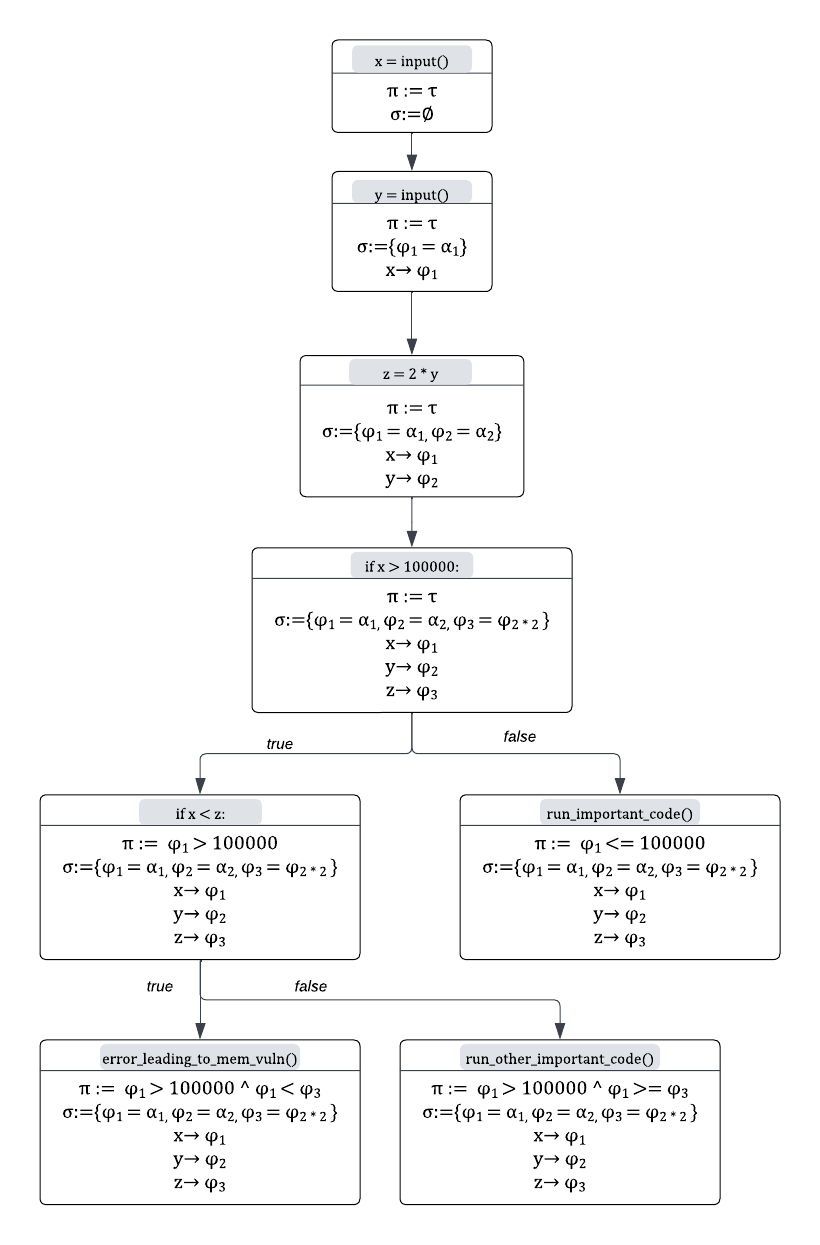
\includegraphics[scale=0.31]{figures/final_symbolic_example_graph.png}
        \caption{} % används för rendera b) som caption
        \label{fig:symbex_example_graph}
    \end{subfigure}

    \caption{Exempel för att visa symbolisk exekvering: pseudokod (a) och path
        constraint och symboliskt tillstånd för alla vägar i pseudokoden angett
        i (b). $  \mathcal{S} = \{\sigma := \{\phi_1 = \alpha_1, \phi_2 = \alpha_2, \phi_3 =
            2\phi_2\}, x \rightarrow \phi_1, y \rightarrow \phi_2, z \rightarrow
            \phi_3\}$}
\end{figure}

Exempelprogrammet i figur~\ref{fig:symbex_example_code} använder symbolisk
exekvering för att hitta vilken indata som leder programexekveringen till de
olika grenarna i programflödet. I många fall är det intressant att göra en
uttömmande sökning och hitta alla möjliga vägar i ett program, något som är
möjligt i detta program men inte i alla. Ett motexempel är komplexa
program som på grund av vägexplosionsproblemet inte hittar alla möjliga vägar.
Variablerna \emph{x} och \emph{y} sätts till symboliska värden som sedan används
för att beräkna vägvillkoret och de symboliska uttryck som variablerna utvecklas
till för en vald gren. Därefter används dessa uttryck och vägvillkor
tillsammans för att bilda en ekvation som sedan kan lösas med hjälp av en SMT-lösare.
Figur~\ref{fig:symbex_example_graph} visar
hur det symboliska tillståndet förändras för alla möjliga grenar i programmet.

I~\ref{fig:symbex_example_graph} används $\pi$ för att ange vägvillkoret vilket
är initialt satt till $\top$ eftersom villkoret är sant från början och $\sigma$
används för att visa mappningen för symboliska värden. $\pi$ och $\sigma$ % något man kan använda ist för mappning kanske
populeras längs med exekveringen, och \emph{x} och \emph{y} mappas till
symboliska värden. Beroende på vilken väg som väljs i exekveringen, uppdateras
vägvillkoret. I andra noden sett uppifrån finns det två skillnader i jämförelse
med den första noden: \emph{x} tilldelas $\phi_1$ som är en symbolisk mappning
till $\alpha_1$. Efter den fjärde noden sett uppifrån görs ett val och
vägvillkoret förändras beroende på vilken väg som tas -- vägvillkoret uppdateras
till $\phi_1 > 100000$ om $x < z$ och annars uppdateras det till $\phi_1 \leq
    100000$. På samma sätt uppdateras $\pi$ och $\phi$ längs andra exekveringsvägar
och vilket till slut leder till ett komplett programflödesdiagram som beror på
\emph{x, y, z}. I varje nod kan ett konkret värde som uppfyller vägvillkoren evalueras.
